\chapter{Umsetzung}
\section{Rekonstruktion und Migration der Simulationsumgebung}
Der Quellcode der alten Arbeit liegt auf GitHub\footnote{\url{https://github.com/MobMonRob/HindernisumfahrungRLStudien/tree/1c0a884c2133107562e4928bfa8bef2ee6e2ade0}} vor.
Im ersten Schritt wird angestrebt, diesen Arbeitsstand zu rekonstruieren, sodass ein Training in der Unity-Umgebung möglich ist.

\subsection{Programmversionen}
Zur Projektbasis liegt neben der Ausarbeitung in \cite{waidner.2020} nur Quellcode vor.
Leider werden dabei die verwendeten Programmversionen nicht dokumentiert, welche jedoch notwendigerweise fein aufeinander abgestimmt sein müssen, um ein Training zu ermöglichen und dessen Erfolg zu gewährleisten.
Sowohl Unity als auch ML-Agents und das zugehörige Python-Toolkit wurden seit der Durchführung von \cite{waidner.2020} in unterschiedlicher Geschwindigkeit weiterentwickelt.
Aufgrund von auftretenden Inkompatibilitäten empfiehlt es sich daher, zunächst die Originalversionen aufzusetzen und dies als Ausgangspunkt für weitere Anpassungen zu nutzen.
Die Unity-Projektdatei enthält Informationen über die exakte Unity-Version, die zur Erstellung des Projekts verwendet wurde.
Leider fehlt jedoch Dokumentation zur verwendeten Version von ML-Agents und des Python-Toolkits.
Recherche in der Veröffentlichungshistorie von ML-Agents ergeben, das höchstwahrscheinlich Version 0.14.1 des Unity-Plugins verwendet wurde.
Daraus ergeben sich Python-Abhängigkeiten, die darauf hindeuten, dass eine Python Version \textgreater= 3.6 und \textless 3.7 verwendet wurde.
Leider gestaltet sich der Versuch erfolglos, diese Versionen auf den verwendeten Entwicklungssystemen (OS X und Linux) zu installieren.
Somit ist es auch nicht möglich, die exakte Entwicklungskonstellation von \cite{waidner.2020} zu rekonstruieren.

Um die Ergebnisse dieser Arbeit möglichst nachhaltig zu machen, soll zur weiteren Entwicklung die aktuelle Version von ML-Agents verwendet werden (Unity-Paket in der Version 2.0.1, Stand: Mai 2023).
Das korrespondierende Python-Plugin ist \code{mlagents} in der Version 0.30.0.
(Zum Zeitpunkt des Schreibens ist es notwendig, das Paket \code{protobuf} in der Version 3.20.3 explizit zu installieren, da sonst die Installation von \code{mlagents} scheitert.)
Die Dependencies dieses Pakets bedingen, dass als neuste Python-Version 3.10.8 verwendet werden kann, welche auch zur Entwicklung gewählt wird.

(Installation und Management spezifischer Patch-Versionen von Python kann kompliziert sein, da in der Regel ein Versionsmanagement nur anhand der Minor-Versionen vorgesehen ist.
Im Rahmen dieser Arbeit hat sich der Einsatz des Programms \code{pyenv}\footnote{\url{https://github.com/pyenv/pyenv}} empfohlen, da sich damit sehr einfach spezifische Versionen von Python individuell kompilieren und managen lassen.)

Da es einerseits Problematiken bereiten kann, neue Plugins mit einer alten Version von Unity zu betreiben und zusätzlich die damals verwendete Version massive Fehler in Kombination mit OS X aufweist, wird auch Unity auf eine aktuelle Version angepasst.
Dafür wird in diesem Fall die aktuellste LTS-Version zum Zeitpunkt der Entwicklung verwendet (2021.3.21.f1).

\subsection{Änderungen der Codebasis}
Da es sich bei ML-Agents um ein vergleichsweise neues Toolkit handelt, unterliegt es fortlaufend einer starken Entwicklung.
Im Zeitraum seit der Vorgängerarbeit wurde das Plugin von einer Alphaversion zu einem offiziellen Release gebracht.
In diesen Entwicklungsphasen kommt es bei Software häufig zu Breaking Changes.
Auch bei ML-Agents ist dies der Fall und es kommt umgehend zum Kompilierungsfehlern, wenn das Unity-Projekt im Editor geöffnet wird.
Der erste Schritt besteht deshalb darin, herauszufinden, welche Methoden davon betroffen sind.
Dafür werden im Fehlerbericht die Methoden gesucht, die Fehler enthalten.
Die Methodenköpfe können dann in die Versionshistorie von ML-Agents\footnote{\url{https://github.com/Unity-Technologies/ml-agents/releases}} gesucht werden.
Im vorliegenden Fall sind somit alle an der Schnittstelle des Toolkit vorgenommenen Änderungen deutlich aufgeschlüsselt und geben Aufschluss darüber, wie die Kompatibilität des Quellcodes wiederhergestellt werden kann.

Für das Training wird in \cite{waidner.2020} eine Trainer-Config-YAML-Datei verwendet, wie sie in \autoref{sec:training} beschrieben wird.
Mit einer Aktualisierung des Python-Toolkits hat sich auch das Format dieser Datei verändert, weshalb die ursprüngliche Datei nicht mehr kompatibel zum nun verwendeten Tooling ist.
Die Änderungen am Format sind vergleichsweise gering und die Datei von überschaubarer Größe, weshalb nach dem Vorbild der alten Datei und unter Anleitung von \cite{mlagentsHyperparameter} die Datei neu gebaut werden kann.
Der Codestand ist nach diesen Veränderungen\footnote{\url{https://github.com/MobMonRob/HindernisumfahrungRLStudien/tree/ec8abbd161217c9a42adb42779e01c5b3dfeb209}} nun mit den aktualisierten Versionen des Toolings kompatibel und wird als Ausgangspunkt für die Experimente dieser Arbeit verwendet.

\subsection{Durchführung des Trainings}
Um ein Training in der Simulationsumgebung durchzuführen wird zuerst eine kompilierte Binary der Trainingsumgebung erstellt.
Zwar ist es theoretisch möglich, direkt aus dem Unity-Editor das Training zu starten.
Allerdings bringt dies einige Nachteile mit sich, wie etwa mangelnde Skalierbarkeit und Performanceverluste.
Außerdem ist es so nicht möglich, das Training effizient auf einer unabhängigen Maschine durchzuführen, die eine weit höhere Trainingsrate ermöglicht.
Um eine solche Binary zu erstellen, wird der Build Prozess in Unity unter File \textgreater Build Settings \textgreater Build gestartet.
Dabei kann die gewünschte Zielplattform ausgewählt werden -- in Abhängigkeit, wo das Training durchgeführt werden soll.
Zum Cross-Compiling ist es allerdings vorausgesetzt, dass die entsprechenden Erweiterungen und Bibliotheken bei der Installation von Unity ausgewählt und geladen wurden.
Sonst ist standardmäßig nur das Kompilieren für die Architektur und Plattform möglich, unter der der Editor ausgeführt wird.

Auf der Maschine, auf der das Training durchgeführt werden soll, muss dafür lediglich das Python-Toolkit installiert sein.
Eine Installation von Unity ist dafür nicht erforderlich, was das Auslagern des Trainingsprozesses und somit ein effizientes Training deutlich vereinfacht.
Für die Experimente im Rahmen dieser Arbeit wird ein virtuelles Rechencluster mit einer Intel Xeon (Gold 6240) CPU mit 8 Kernen, einer Nvidia vGPU V100D-8C und Ubuntu 20.04.1 LTS zum Einsatz.
Deshalb wird das Environment für Linux x86\_64 gebaut und es ist kein Cross-Compiling von der Entwicklungsmaschine zur Trainingsmaschine nötig.
Unity produziert bei Kompilierung für Linux einen Ordner mit den Ausgabedateien, welche sowohl die eigentliche Binary als auch Artefakte und Libraries enthalten.
Dieser Ordner sollte deshalb vollständig auf die Trainingsmaschine übertragen werden.
Für die Durchführung des Trainingsprozesses können verschiedene Parameter von \code{mlagents-learn} angepasst werden.
Es ist keine pauschale Angabe möglich, welche Parameter verlässlich und auf allen möglichen Trainingsmaschinen zu einem guten Ergebnis führen.
Deshalb ist eine kleine Testreihe unerlässlich, bei der möglichst gute Werte für die Parameter ermittelt werden, um das spätere Training effizient zu gestalten.
Der maßgebliche Performanceindikator ist hierbei die Anzahl der Trainingsschritte pro Sekunde.
Zur Optimierung wird beispielsweise nach und nach die Anzahl der parallelen Trainingsumgebungen erhöht, bis die Anzahl der Schritte pro Sekunde nicht mehr weiter steigt.
Die nachfolgende Befehlszeile scheint nach einigem Optimieren gute Ergebnisse für die Machienenkonfiguration zu liefern:
\code{mlagents-learn --env binary-name/binary-name.x86\_64 --run-id run-name --no-graphics --torch-device cuda --num-envs 4 --time-scale 1 trainer.yaml}.
Dabei werden 4 parallele Trainingsumgebungen (mit jeweils 30 Agenten) ohne Generierung von grafischen Artefakten betrieben.
ML-Agents greift intern auf Tensorflow und PyTorch zurück.
Grundsätzlich bieten beide Bibliotheken die Möglichkeit, eine CUDA-fähige GPU zur Grafikbeschleunigung der Trainingsalgorithmen zu verwenden.
Im Kontext des verwendeten Trainingsalgorithmus (\ac{ppo}) ist infrage zu stellen, ob ein ernstzunehmender Vorteil durch die Verwendung einer GPU erzielt werden kann.
Ressourcen im Internet sind sich hierüber uneinig.
Da es jedoch nicht zu einer Verschlechterung und bestenfalls zu einer Verbesserung kommen kann, und die GPU zur Verfügung stand, wird sie dem Trainingsprozess auch als Ressource zur Verfügung gestellt.
Weiterhin wird die Wahl getroffen, die \code{time-scale} des Trainingsprozesses auf 1 zu setzen.
Standardmäßig wird dieser Parameter von ML-Agents auf 20 gesetzt, was den Trainingsprozess beschleunigen soll.
Vergleichende Tests ergeben jedoch, dass es im Kontext der verwendeten Trainingsumgebung und Trainingsmaschine keinen Unterschied für die Geschwindigkeit der Trainingsoperationen zu machen scheint, auf welchen Wert der Parameter gesetzt wird.
Es gibt jedoch Hinweise, dass bestimmte Arten von physikalischen Berechnungen von der zeitlichen Skalierung beeinflusst werden \cite{zhang2021}.
Da unklar ist, ob solche Berechnungen hier Verwendung finden und gegebenenfalls sogar eine Ursache für die eigenartige Fortbewegungsart des Roboters im bisherigen Training sein könnten, wird für das Training, wie bereits erwähnt, eine nicht-verzerrte Zeitskala verwendet.
(Da jedoch der Parameter die Schritte pro Sekunde nicht zu beeinflussen scheint, ist zu hinterfragen, ob er in der verwendeten Version der Toolkits überhaupt korrekt interpretiert wird.)

\begin{figure}[H]
    \centering
    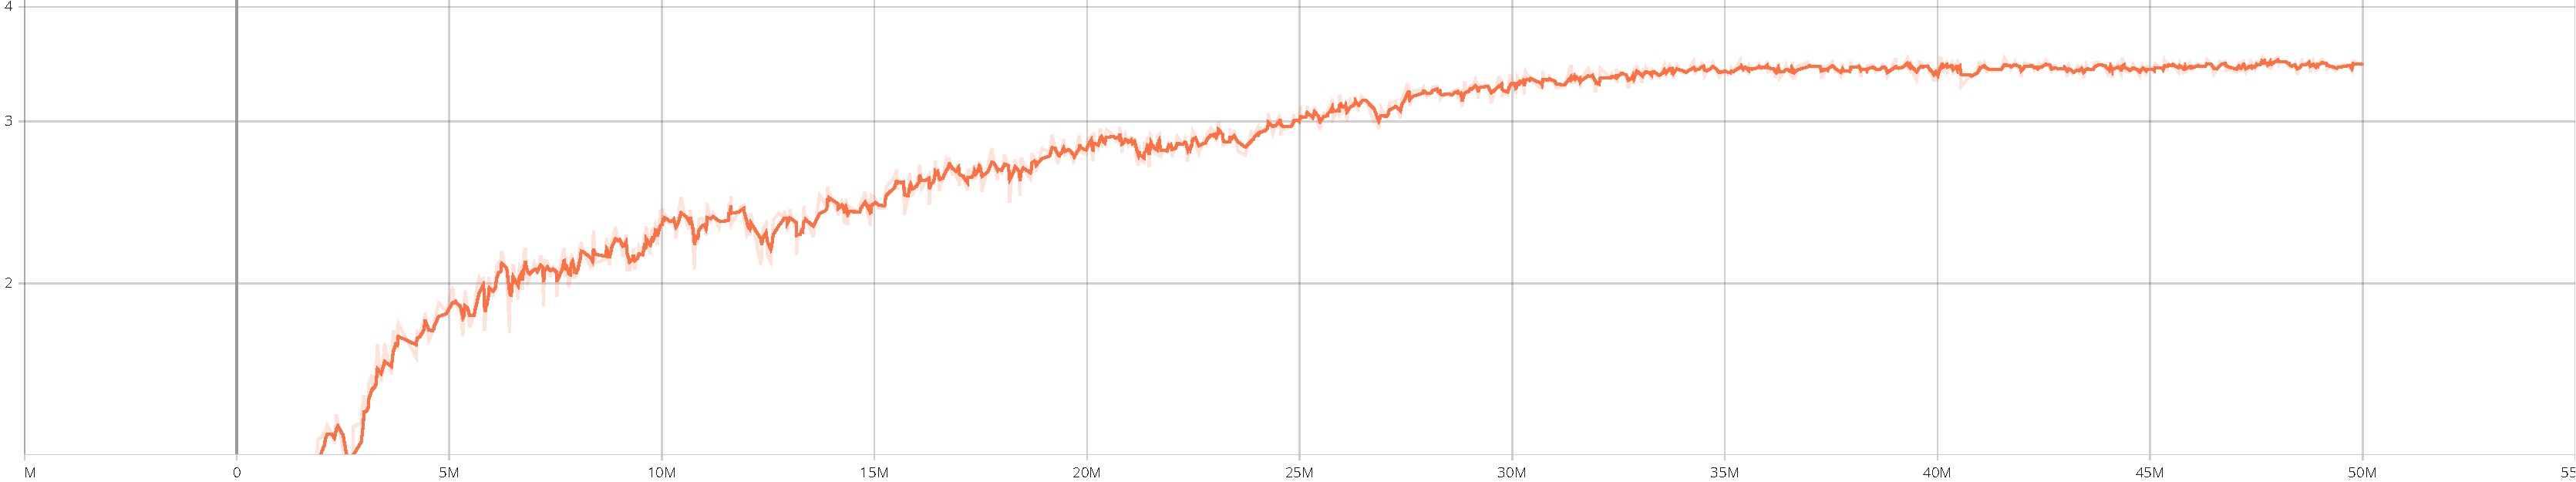
\includegraphics[width=\textwidth]{Bilder/ml-agents/Environment_Cumulative Reward_time-scale-1.pdf}
    \caption{Cumulative Reward der Rekonstruktion von \cite{waidner.2020}}
    \label{fig:time-scale-1}
\end{figure}

Der Verlauf des Cumulative Rewards, der nun beim Training entsteht und in \autoref{fig:time-scale-1} dargestellt wird, gleicht im Wesentlichen den Resultaten von \cite[50]{waidner.2020}.
Auch der gelernte Bewegungsablauf, der bei der Inferenz zu beobachten ist\todo{Video}, gleicht den Resultaten der vorangegangenen Arbeit, weshalb die Rekonstruktion als erfolgreich bewertet wird.


\section{Stabilisierung des Laufverhaltens}
Wie in \autoref{sec:probleme} ausgeführt und von den Ergebnissen der Rekonstruktion zusätzlich veranschaulicht wird, bewegt sich der Roboter aktuell mit einer sprungartigen Bewegung fort.
Diese ist, wie beschrieben, Ursache für viele potenzielle Probleme.
Deshalb soll nun das Laufverhalten stabilisiert werden.
In diesem Zusammenhang wird darunter verstanden, die Schwankungen, die die Körpermitte bei der Bewegung vollführt, auf ein Minimum zu begrenzen.
Wird das Vorbild der Spinnen betrachtet, so ist davon auszugehen, dass diese Einschränkung kein Hindernis für eine effiziente Fortbewegung darstellt.

Es existieren innerhalb der Simulation zwei elementare C\#-Skripte, die für die in diesem Kapitel beschriebenen Änderungen von besonderer Relevanz sind: \code{SpiderAgent.cs} und \code{SpiderController.cs}.
In \code{SpiderAgent.cs} befinden sich die für den Reinforcement Learning Prozess relevanten Konfigurationen des Agenten.
Dort werden Beobachtungen gesammelt und dem Lernalgorithmus zur Verfügung gestellt, die Aktionen vom Lernalgorithmus entgegengenommen, die Lern-Episoden verwaltet und vor allem der Reward zugewiesen.
Der \code{SpiderController} ist wiederum einem \code{SpiderAgent} zugeordnet und verwaltet dessen Skripte für die Servomotoren, koordiniert die allgemeine Durchführung der Bewegung und führt das Zurücksetzen der Komponenten durch.
Da ein \code{SpiderController} somit auf die direkten Werte des Roboterzustands zugreifen kann, wird hier auch der Reward berechnet, der in \code{SpiderAgent.cs} zugewiesen wird.

Für die Stabilisierung der Bewegung bestehen nun zwei verschiedene Ansätze, die ausprobiert und verglichen werden.
Beide werden über Änderungen in \code{SpiderController.cs} realisiert.
Die dort implementierte, allgemeine Bewegungskoordination des Roboters ist eine seiner physikalischen Grundeigenschaften und wird deshalb im Rahmen dieser Arbeit nicht manipuliert.
Auch wird so eine kontinuierliche Basis für die einzelnen Versuche und deren Evaluation geboten.
Jedoch stellt der in dieser Klasse berechnete Reward die zentralste Stellschraube des Reinforcement Learning Problems dar.

\lstinputlisting[
    % language = C,
    firstline = 8,
    % lastline = 41,
    caption = Ürsprüngliche Berechnung des Reward-Signals,
    label = code:reward-post-reconstruct
]{Code/post-reconstruct/reward.cs}

In \autoref{code:reward-post-reconstruct} ist die ursprüngliche Berechnung des Rewards zu sehen, wie sie in \code{SpiderController.cs}.
Dabei wird zunächst der Reward mit 0 initialisiert.
Anschließend wird abgeprüft, ob sich der Roboter um mehr als 90° zur horizontalen Achse gedreht hat und eine negative Belohnung vergeben, falls dies der Fall sein sollte.
Mit dieser Prüfung soll verhindert werden, dass der Roboter sich überschlägt und dabei seine empfindliche Elektronik beschädigt.
Anschließend wird geprüft, wie weit der Roboter auf der Karte in Vorwärtsrichtung von seinem Ausgangspunkt entfernt ist und die Differenz zum vorherigen Resultat dieser Berechnung gebildet.
Diese Differenz -- sowohl wenn diese positiv ausfällt, als auch, wenn sie negativ ist -- wird dann mit der eventuellen Strafe für ein Überschlagen verrechnet und als Reward zurückgegeben.

Der offensichtliche und einfache Weg ist es nun, in der Methode \code{isTurned()} den Schwellwert der Rückgabe von 90° auf einen kleineren Wert, zum Beispiel 5°, zu reduzieren.
Mit dieser Modifikation wird automatisch ein negativer Summand in den Reward eingebracht.
Das Problem hierbei besteht darin, dass die Methode \code{isTurned()} nicht nur zur Berechnung des Rewards verwendet wird, sondern auch in \code{SpiderAgent.cs} die aktuelle Episode terminiert wird, wenn sich der Roboter auf den Rücken dreht.
Wird die Modifikation an dieser Methode vorgenommen, so wird auch eine kleine Schwankung der Körpermitte als Überschlag interpretiert und die laufende Trainings-Episode fälschlicherweise beendet.
Wie sich bei einem Trainingsversuch zeigt, führt dies dazu, dass der Roboter kein Laufverhalten lernen kann, da ihm keine Gelegenheit geboten wird, seinen Fehler zu erkennen, zu erforschen und zu korrigieren.
Für eine möglichst stabile Körpermitte sollte der Rotations-Schwellwert möglichst gering sein.
Jedoch wird bei diesem Ansatz ein Training gegenläufig zum sinkenden Schwellwert praktisch unmöglich.




\section{Pfadplanung}
\subsection{Proof of Concept: Crawler}
Zeigen, dass es grundsätzlich möglich ist

\subsection{Übertragung auf den SpiderAgent}
Versuche mit verschiedenen Rewards
überhaupt, Neudesign der Rewards, welche Ansätze gibt es hier, wie werden sie implementiert, welche Ergebnisse gibt es dabei

\section{Hindernisumfahrung}
\subsection{Grundsätzliche Experimente}
Training auf Basis von Laufstabilisiertem Stand, da Pfadplanung mit dem Roboter noch nicht funktioniert
statisches Hindernis
Roboter läuft Kurve und lernt Existenz und Position von Hindernis auswendig
\subsection{Crawler-Versuche}
mit vorhandenem Modell und Pfadplanung, allerdigns nicht extra dafür trainiert
wäre komisch, wenn es funktioniert, aber zeigt auch, dass ein gesondertes Training notwendig ist